\chapter{Methods} \label{sec:methods}

The main objective of this work is to find out to what extent the synthetic images generated by text-to-image models are usable in real tasks in the field of computer vision. Therefore, the main contribution of this work consists of creating a pipeline that allows the use of synthetic images in the training of deep learning models. In addition, this paper includes extensive experimentation to show how effective this approach is.

\section{Subject-driven augmentation} \label{sec: sdAugmentation}

The developed pipeline responds to the need to implement the novel task of \textit{subject-driven augmentation}. The idea behind this concept is to use subject-driven generation techniques to generate new subject images to augment datasets of computer vision tasks. At the time of writing, there are no implementations for this novel data augmentation technique in the leading deep learning libraries. Therefore, we have chosen to build the pipeline from scratch.

Considering a dataset divided into classes, one of them is taken. Then, 3 to 5 images are randomly selected. The next step is to apply the subject-driven technique to obtain a modified text-to-image model. In this way, the customised model will be able to generate synthetic images of the subject or class under consideration. By adding these images to the training set of a successive task, the original images are automatically augmented. This approach is called \textit{subject-driven augmentation}. Figure \ref{fig:subjectDrivenP} shows a schematic of the developed pipeline.

\begin{figure}
    \centering
    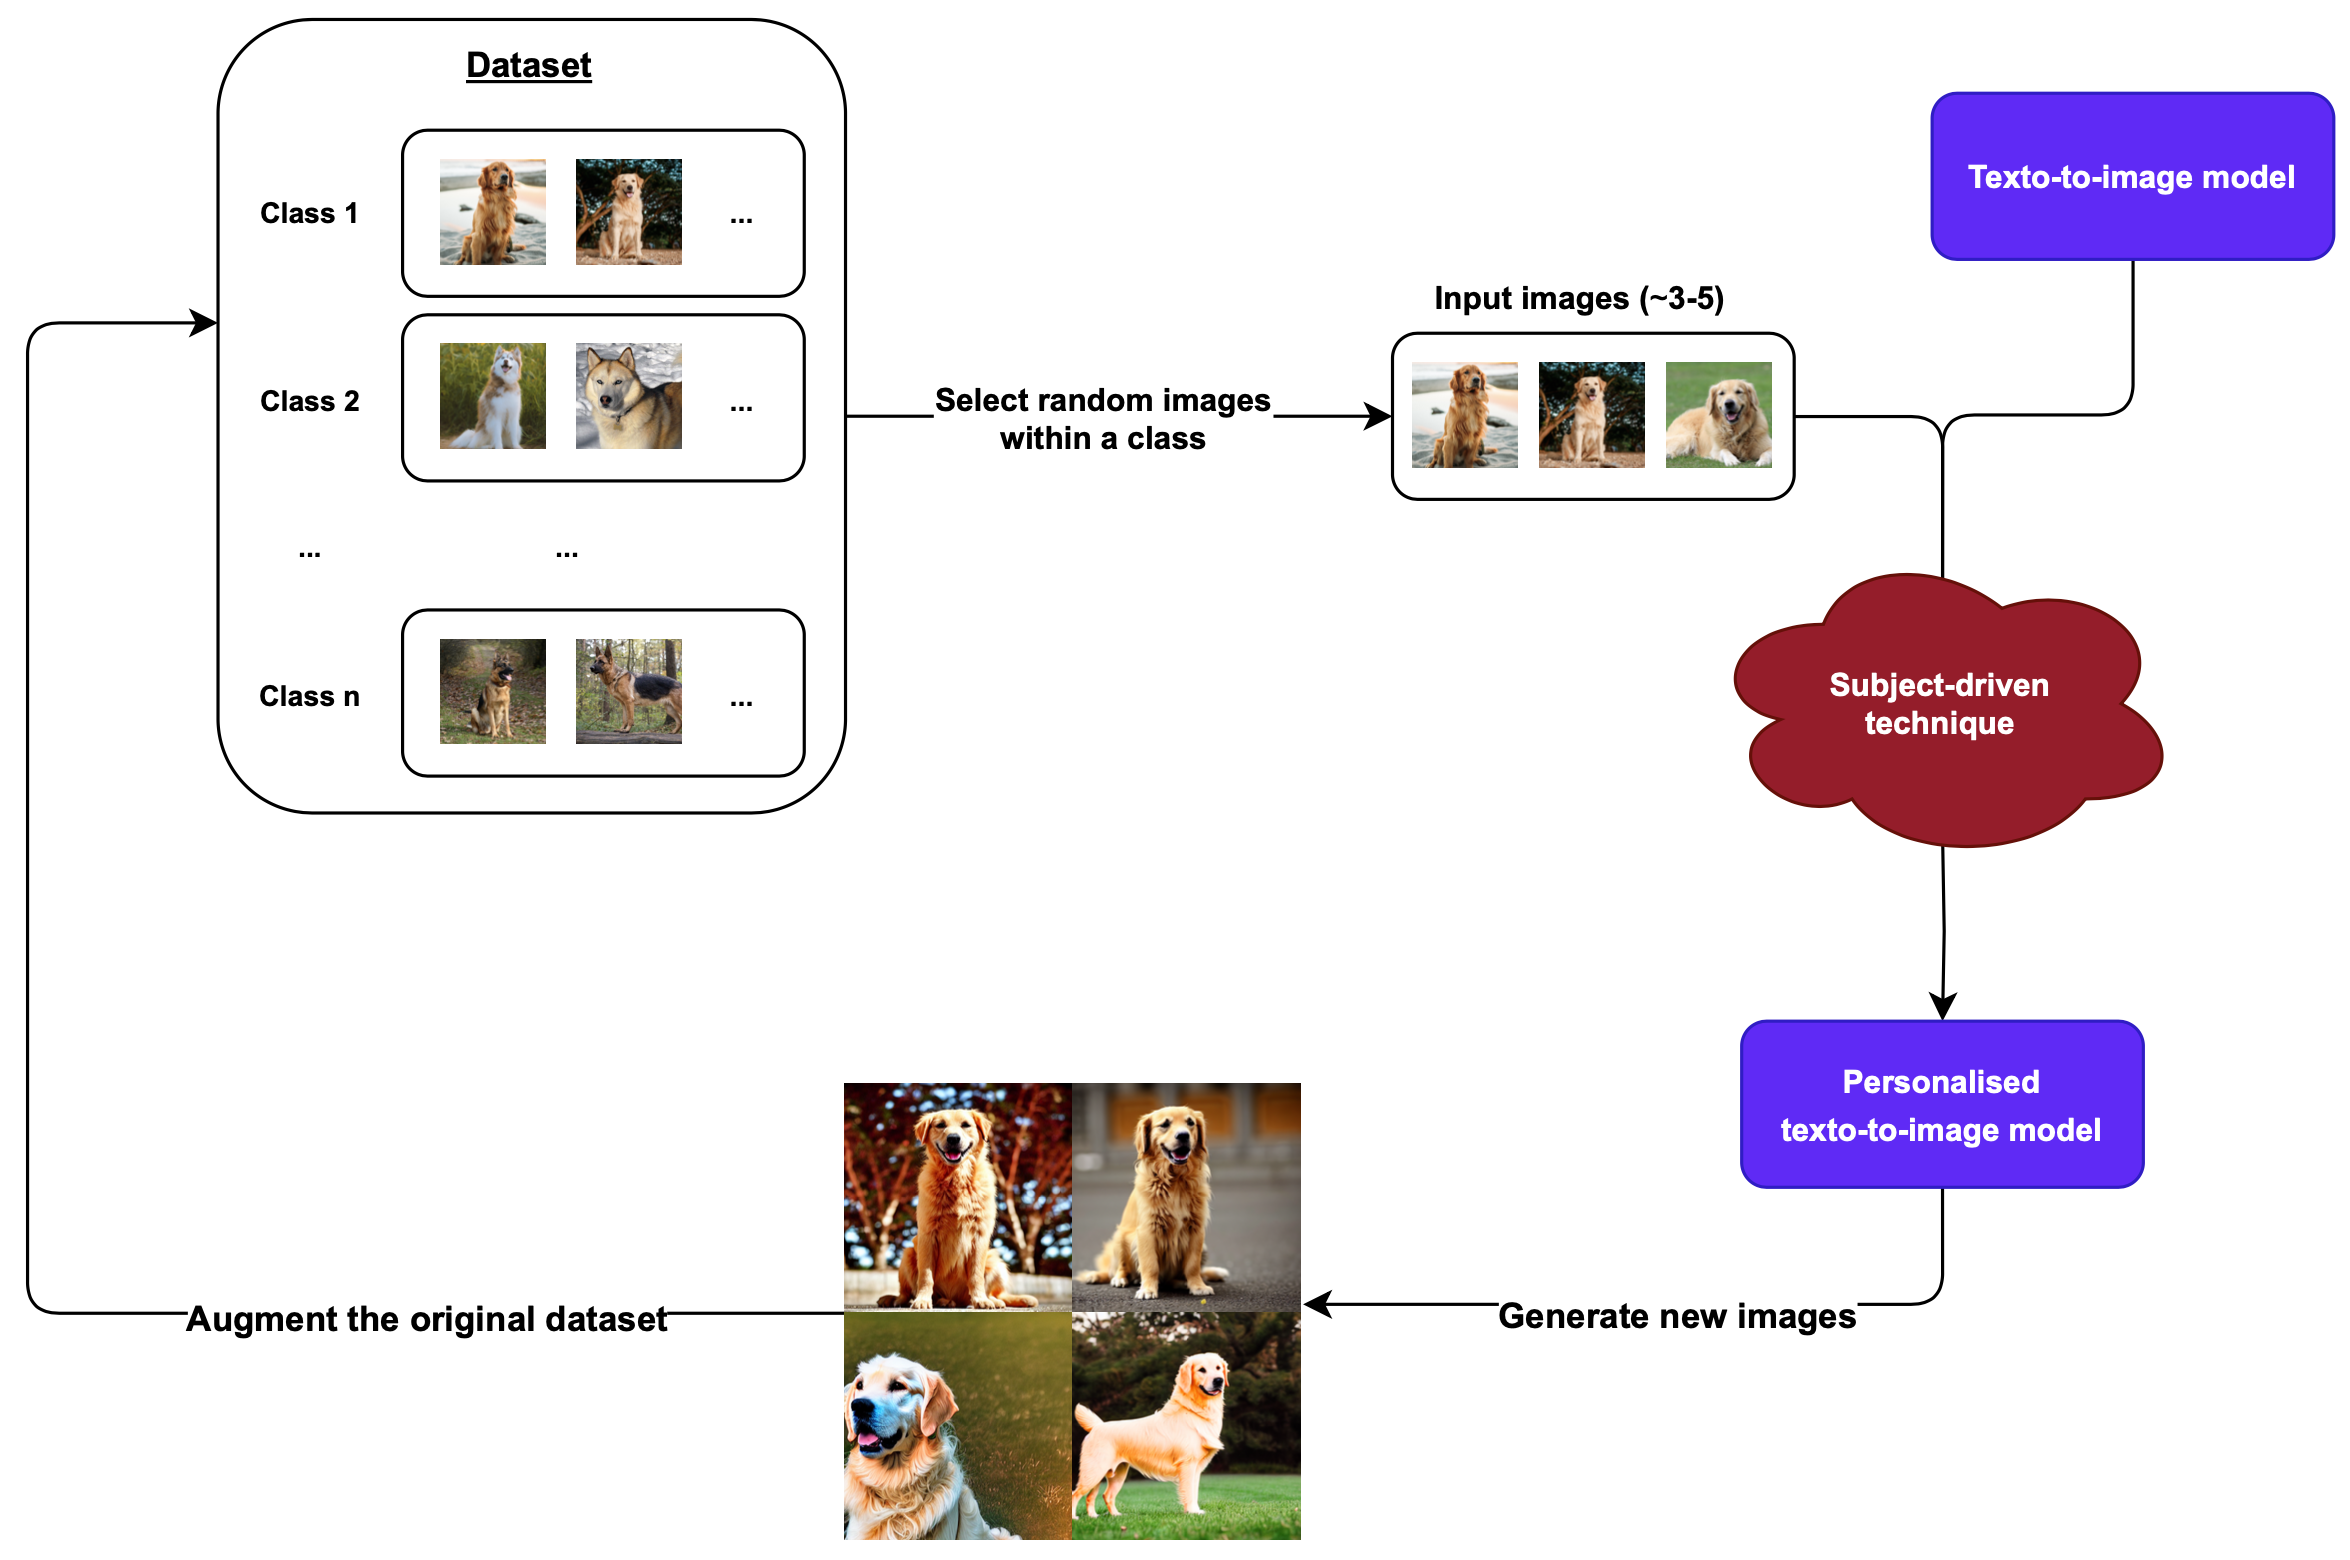
\includegraphics[width=0.9\textwidth]{Pictures/subjectDrivenP.png} 
    \caption{\textbf{Subject-driven augmentation schema}.  It proposes selecting 3-5 images from each class. Then, the subject-driven technique helps to generate synthetic images of subjects within the class considered. By adding those images to the dataset, it gets augmented.}
    \label{fig:subjectDrivenP}
\end{figure}

Dreambooth and Textual inversion are used as subject-driven generation techniques. Both strategies allow the developed pipeline to be generalist, and they allow it to be applied in a wide range of scenarios. However, it is a complex approach that requires customising a text-to-image model for each of the classes contained in the considered dataset. In the case of Dreambooth, fine-tuning of the model is necessary. On the contrary, in Textual inversion, the embedding token must be found for a new token corresponding to the considered subject. Thus, if we want to augment a dataset with a large number of different classes, we will need a significant amount of time. Therefore, we propose a solution using the image generation model directly. For this purpose, we only use the names of the classes used to build the dataset. Thus, we build a prompt with it and directly generate images of the considered class.

This approach solves the problem of customising the text-to-image model and thus reduces the amount of time required to augment the dataset. However, using only the class name has a fundamental problem. The image generation model may not have enough information to be able to generalise images of certain classes. This will, of course, depend on how sparse the presence of objects of the class is in the training set of images of the text-to-image model. Thus, with classes that represent common objects and that are certain to have participated in a relevant way in the training of the model, there will be no complications. On the contrary, if working in a non-common domain, the images generated with this approach will not be of sufficient quality to be part of the augmented dataset. Figure \ref{fig:controlNetP} shows an outline of the pipeline considering only the class name when generating the synthetic images.

\begin{figure}
    \centering
    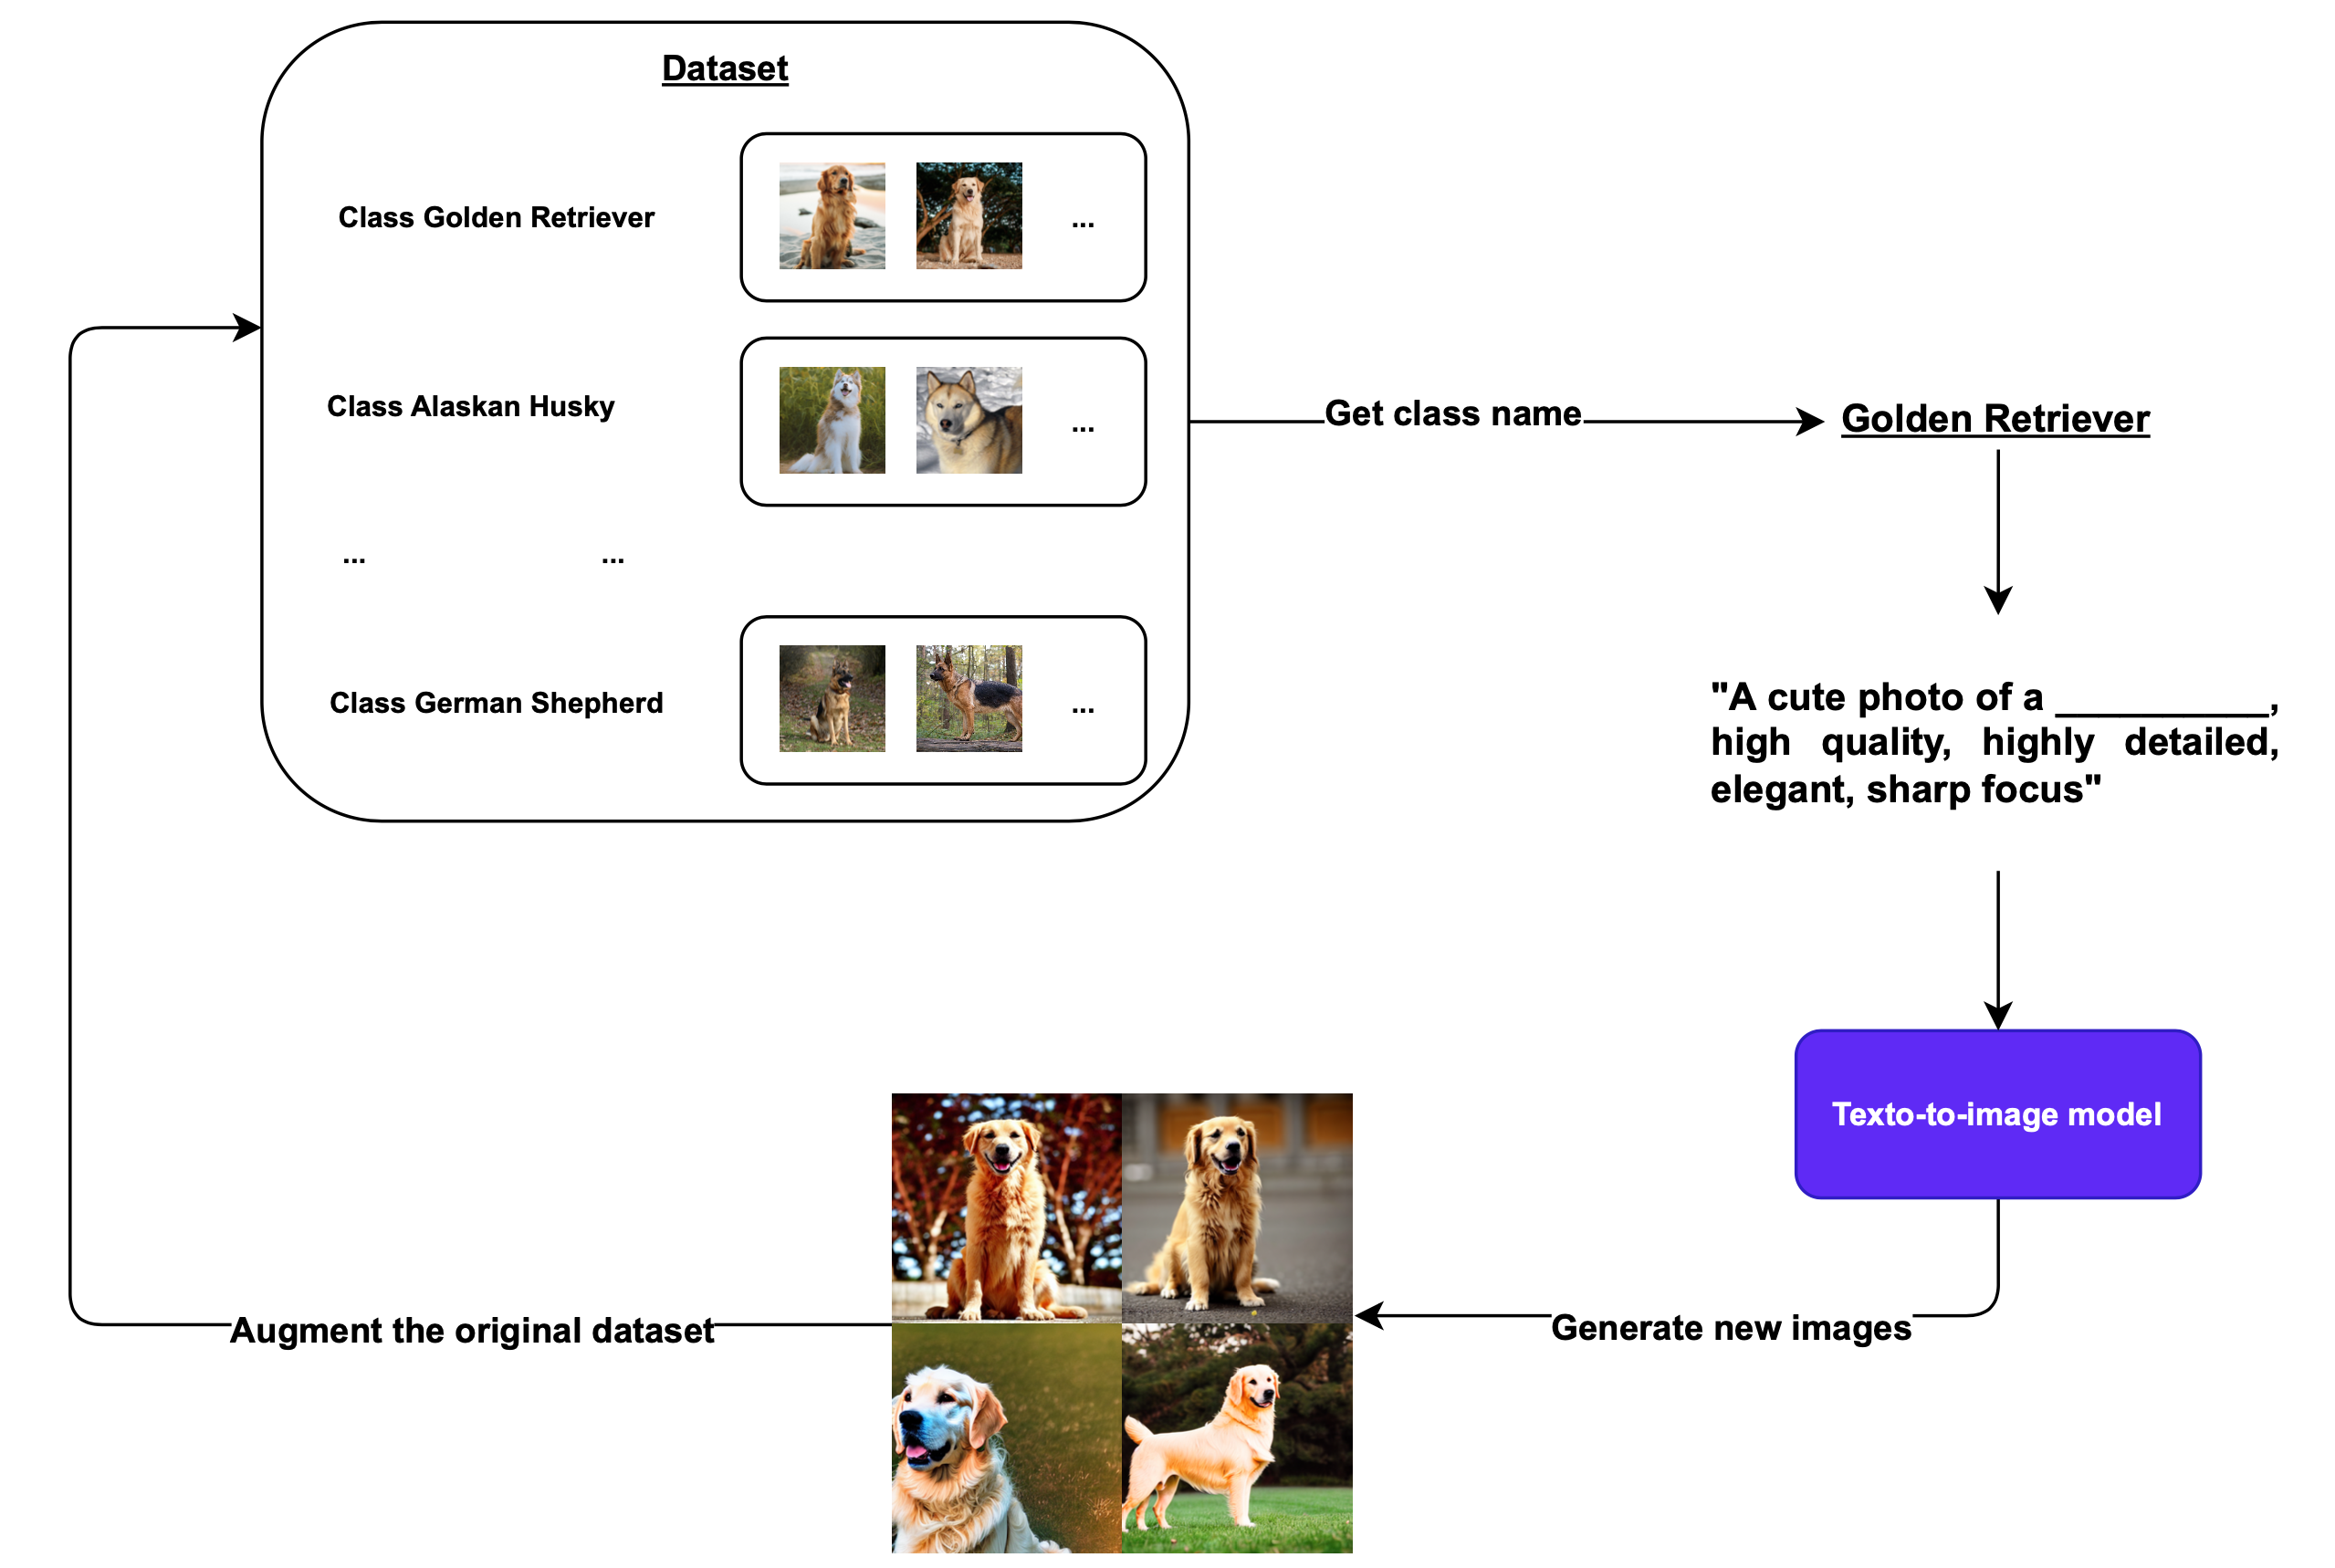
\includegraphics[width=0.85\textwidth]{Pictures/controlNetP.png} 
    \caption{\textbf{Class name-based augmentation schema}. The difference with the subject-driven schema is that the image generation model is used directly. Only the names of the classes used to build the dataset are employed to generate the synthetic images. With the class name, a suitable and general prompt is generated.}
    \label{fig:controlNetP}
\end{figure}

The approach shown for subject-driven augmentation has straightforward applications in computer vision tasks such as classification. However, there is the problem of controlling the generated images. If, for example, we want to apply this approach to a segmentation task, we will find it very difficult to generate subjects with specific poses or arrangements. The reason is that although textual descriptions offer a great deal of flexibility, they have obvious limitations when conveying how the final image should look. We, therefore, consider the use of ControlNet to add conditional control. Taking the pipeline for the class name-based augmentation case, the only thing that needs to be added is conditional control for the text-to-image model. In this way, a control element must be provided for each image to be generated. As we consider a segmentation task, segmentation maps can be provided, although other alternatives, such as Canny edge detections, may also be valid. With this modification, the generated image will have the layout of the provided condition. Therefore, the image can be used with its associated segmentation map to augment the datasets used in segmentation tasks. Figure \ref{fig:controlNetPipe} shows what this strategy looks like.

\begin{figure}
    \centering
    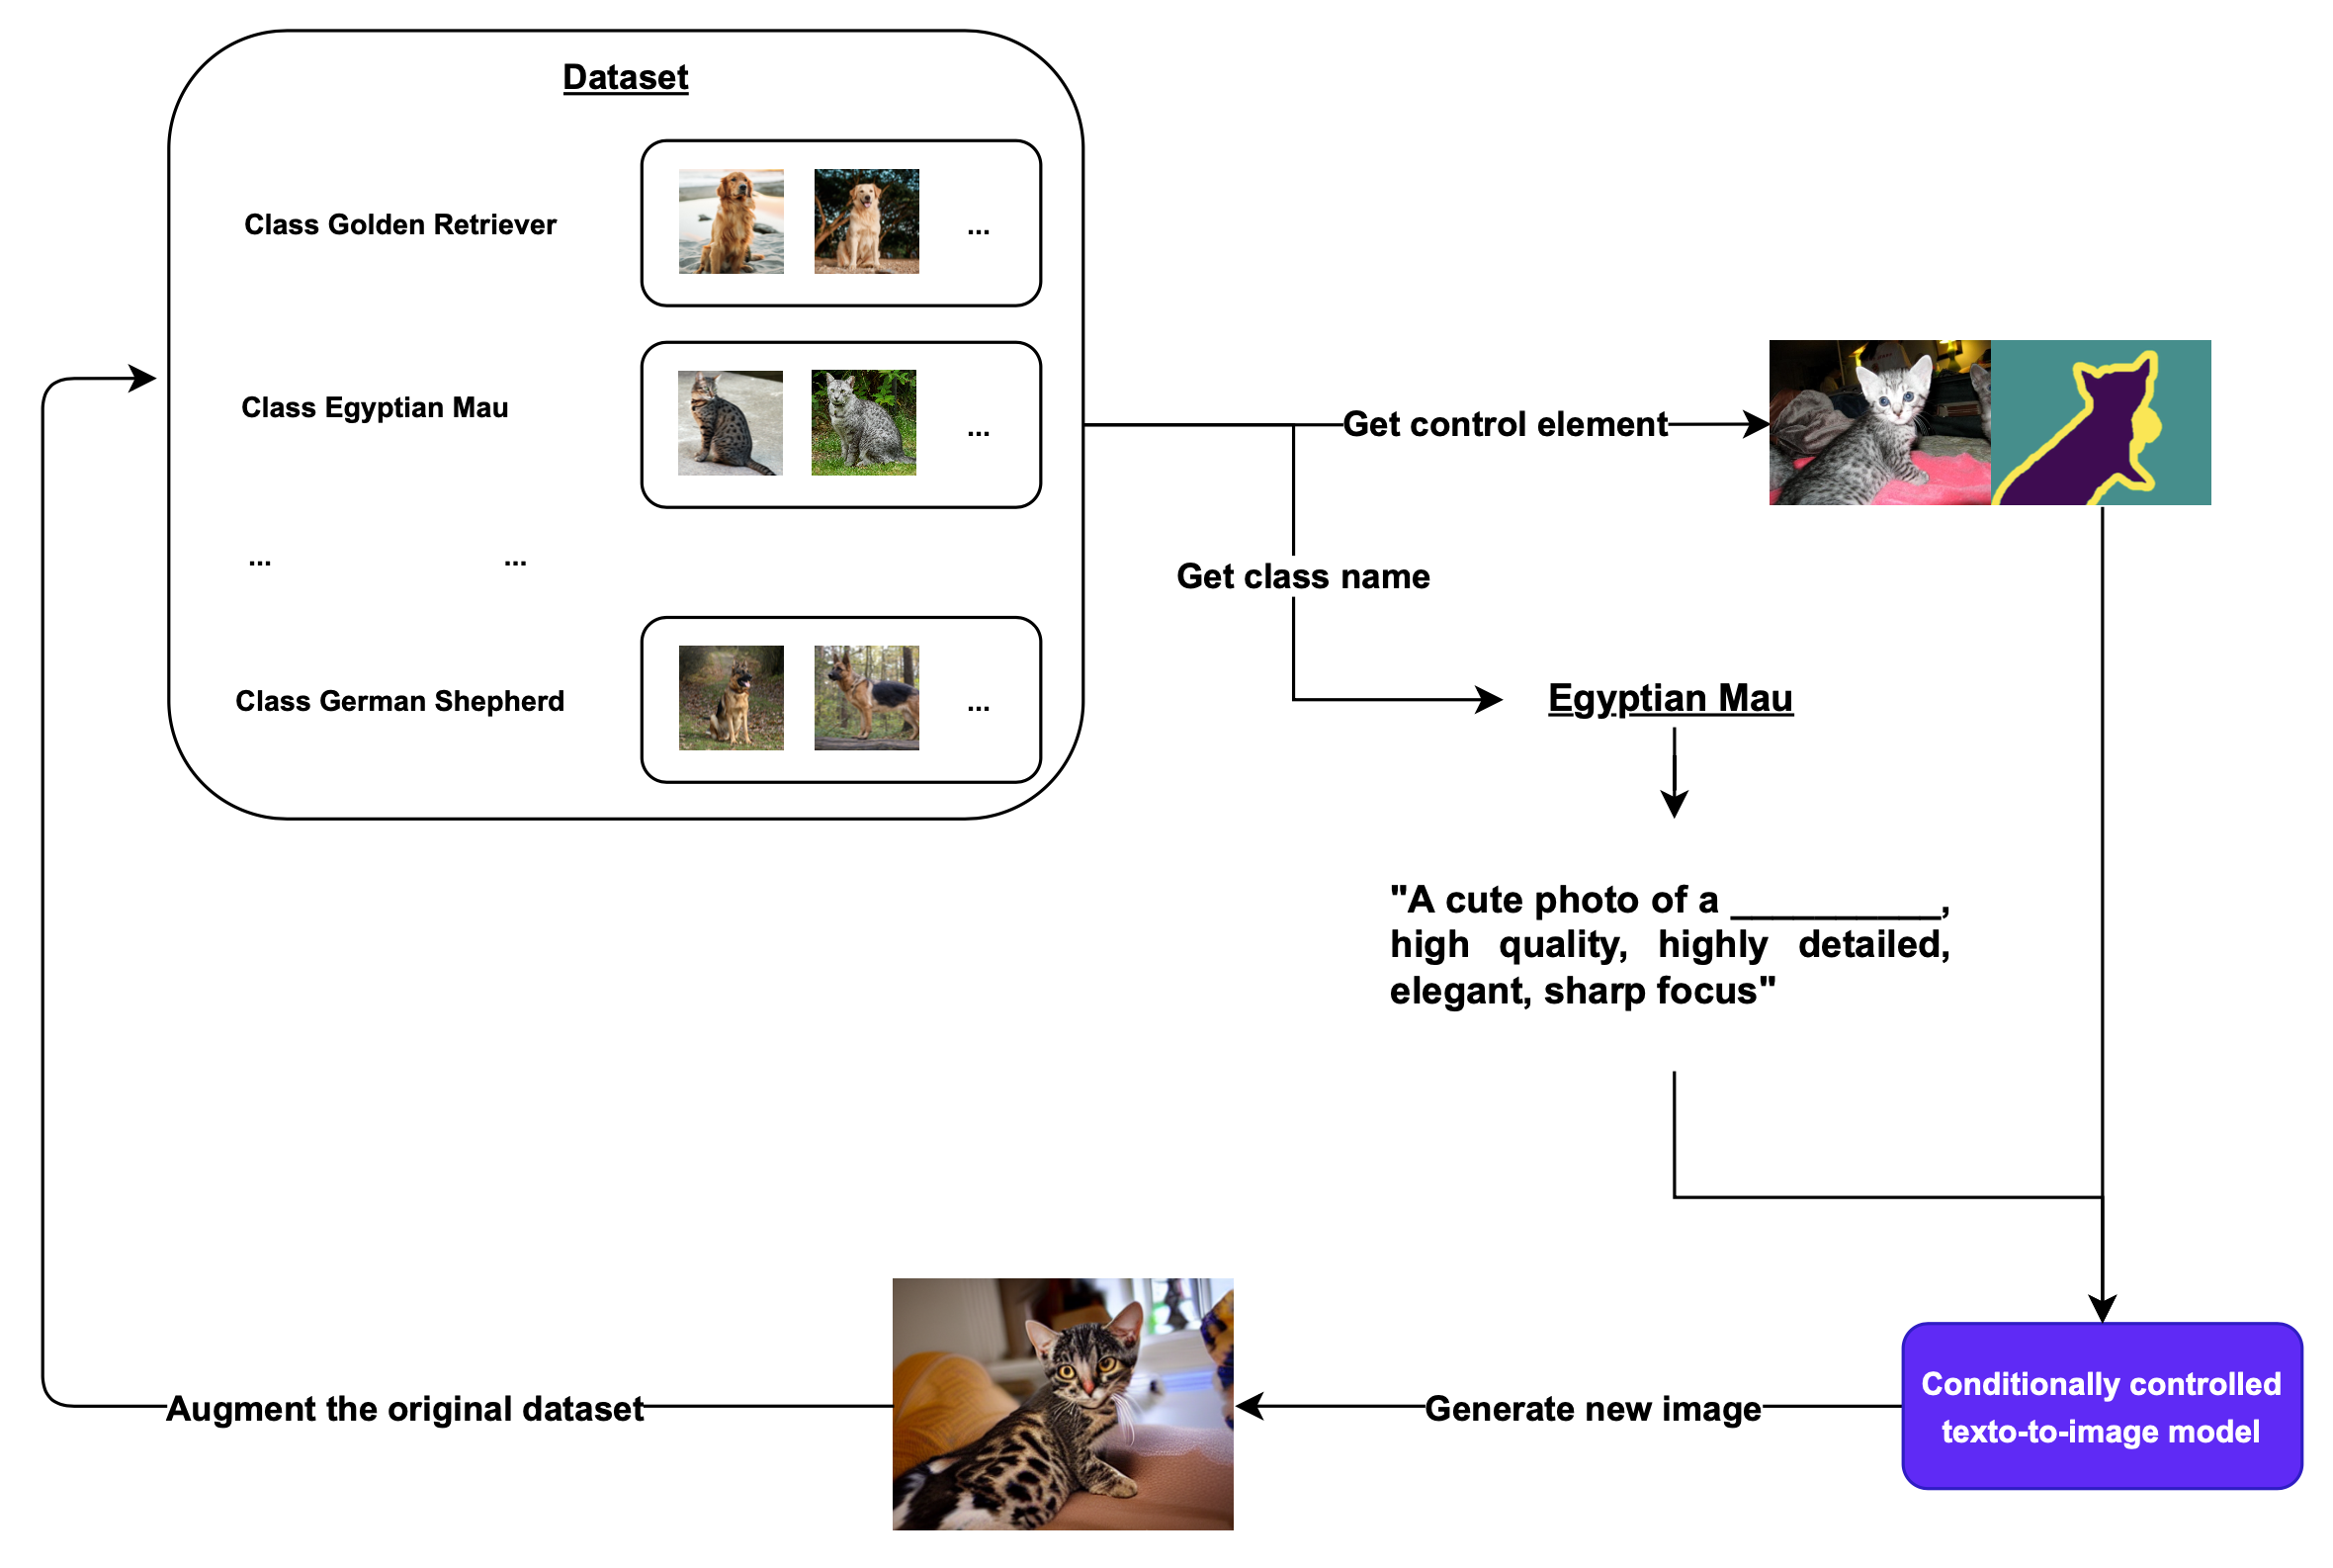
\includegraphics[width=0.85\textwidth]{Pictures/controlNetPipe.png} 
    \caption{\textbf{Augmentation schema using a conditionally controlled texto-to-image model}. In this case, it is also necessary to use a control element in addition to the class identifier. In the case shown, a segmentation map is used; thus, the image generated by the model will share the same map. In this way, augmenting a segmentation task by generating synthetic image and segmentation map pairs is possible.}
    \label{fig:controlNetPipe}
\end{figure}

In summary, the methods developed in this work show how to generate synthetic images to augment datasets in computer vision tasks. Therefore, we present three pipelines using Dreambooth and Textual inversion, class name-based generation, and ControlNet for classification and segmentation tasks.